\documentclass[final]{cvpr}
\usepackage{times}
\usepackage{graphicx}
\usepackage{amsmath}
\usepackage{amssymb}
\usepackage{float}
\usepackage{caption}
\usepackage{tikz}
\usetikzlibrary{positioning,arrows.meta,shapes.geometric,fit,backgrounds}
\usepackage[pagebackref=true,breaklinks=true,colorlinks,bookmarks=false]{hyperref}

\begin{document}

\title{MedBridge: A Policy-Grounded, Tool-Using LLM Agent for Healthcare Prior Authorization and Denial Appeal}

\author{Neha Kumari\\
Northeastern University\\
kumari.neh@northeastern.edu}

\twocolumn[{
    \renewcommand\twocolumn[1][]{#1}%
    \maketitle
    \begin{center}
      \centering
      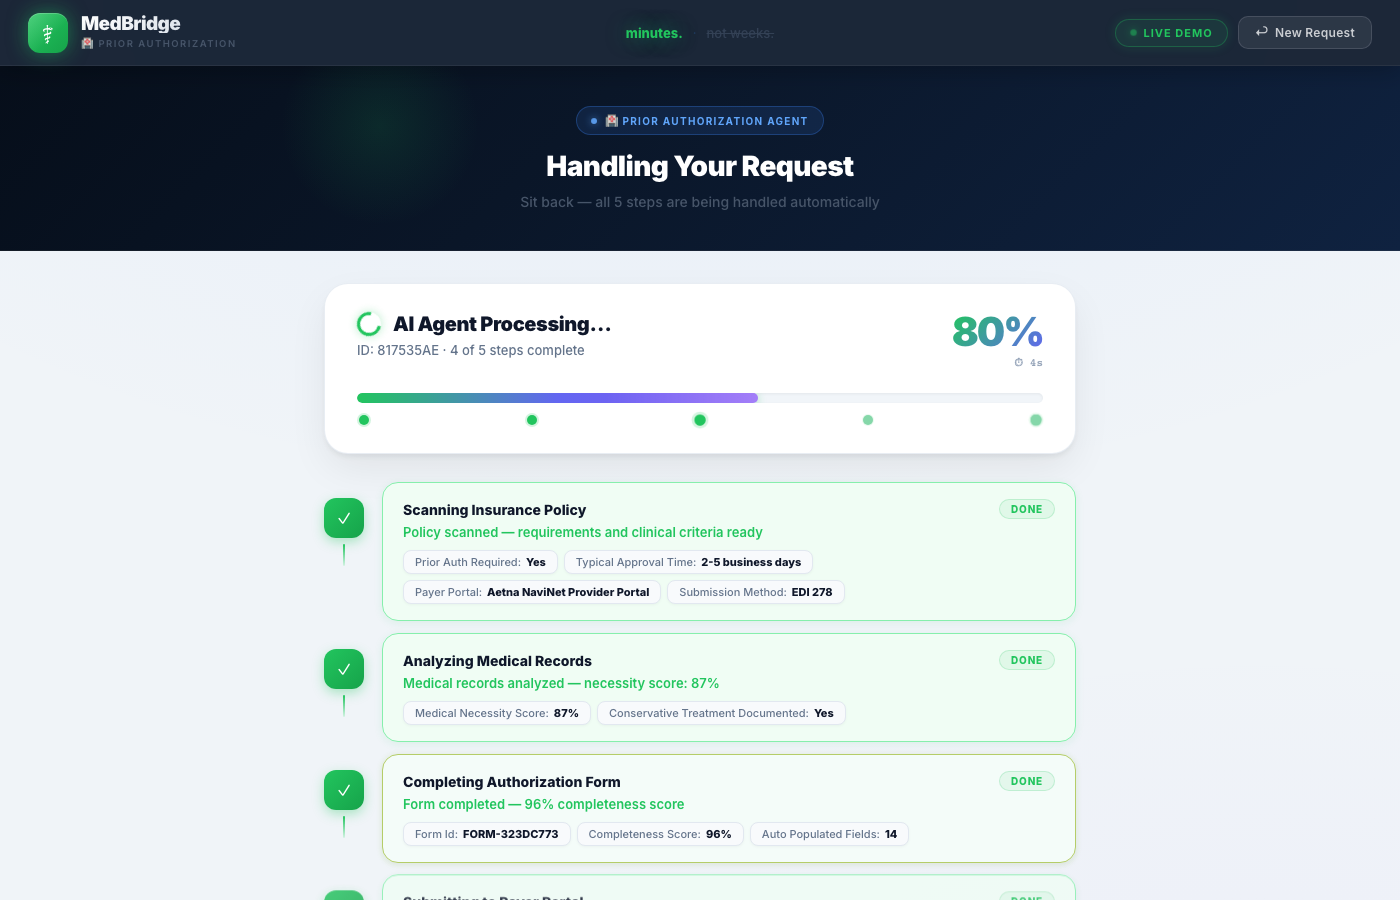
\includegraphics[width=0.8\textwidth]{fig/cover_workflow.png}
      \captionof{figure}{MedBridge web interface: the agent's tool calls (policy scan, record analysis, form fill, submission, status tracking) stream to the user in real time. Screenshot of our own prototype.}
      \label{fig_teaser}
    \end{center}
}]

%-------------------------------------------------------------------------
\section{Abstract}
Prior authorization (PA) requires clinicians to obtain insurer approval before many tests and treatments, a manual, fax-driven process that delays care and is frequently followed by labor-intensive appeals. We present \emph{MedBridge}, a domain-specific chatbot-agent that takes one structured request (patient, payer, treatment, diagnosis, clinical justification) and autonomously runs the PA workflow: it retrieves payer policy criteria with retrieval-augmented generation (RAG), analyzes clinical records, completes the form, pauses for human approval, then submits, tracks the decision and, on denial, drafts an appeal citing the retrieved policy text. The output is a reviewed request with an audit trail, or a cited appeal letter awaiting physician signature. MedBridge targets clinic administrative staff and demonstrates how RAG plus an LLM tool-use loop can reduce administrative burden while keeping every claim traceable to a source.

%-------------------------------------------------------------------------
\section{Introduction}
\noindent\fbox{\parbox{\dimexpr\linewidth-2\fboxsep-2\fboxrule\relax}{\small\textbf{MedBridge won 1st place at the AI Agents Hackathon, hosted by OSS4AI in collaboration with Beta Fund and Gravitational Ventures, and was built solo} \cite{medbridge_hackathon}. This paper describes how that prototype is rebuilt and extended for this course.}}

\smallskip
General-purpose LLMs converse fluently but lack three things a PA assistant needs: (i) current, payer-specific coverage criteria, (ii) the ability to \emph{act} (submit, track, appeal) rather than only advise, and (iii) traceability, since a wrong coverage claim in a submission has real consequences. The burden is well documented. In the American Medical Association's 2024 survey of 1{,}000 physicians, 94\% said prior authorization delays necessary care, 24\% reported a serious adverse event for a patient, and practices reported completing 43 requests and spending about 12 staff hours per physician each week \cite{ama2024} (the AMA opposes prior authorization, so these are advocacy-group survey results). Denials are common and mostly wrong when challenged: in 2024 Medicare Advantage insurers fully or partially denied 4.1 million of 52.8 million requests, yet 80.7\% of appealed denials were overturned, while only 11.5\% of denials were appealed \cite{kff2024}. Waits are contested: in an earlier AMA survey (2017 data) about two-thirds of physicians reported waiting at least one business day for a decision and roughly 30\% three days or longer \cite{ama2018}, whereas insurer-reported metrics show median standard-request response times of about one day \cite{kffmetrics}. Manual handling is costly: in the 2019 CAQH Index a manual prior authorization cost providers \$10.92 against \$1.88 electronically \cite{caqh2019}. This pattern, in which most appealed denials succeed but few are appealed, motivates a tool that drafts well-supported requests and appeals for human review.

MedBridge addresses these gaps with two course techniques: \textbf{Knowledge Augmentation \& Retrieval} (policy documents embedded in a vector database and retrieved per request) and \textbf{Agentic Workflows \& Tool Use} (an LLM-driven loop that chooses among six tools and branches on denial). The prototype was first built as a solo hackathon project that won 1st place; this work extends it by replacing hard-coded policy lookups with retrieval over real payer documents and by defining a quantitative evaluation.

%-------------------------------------------------------------------------
\section{Related Work}
\textbf{RAG.} Lewis \etal\cite{lewis2020rag} combine a parametric generator with a non-parametric retriever to ground outputs in external text. In medicine, Xiong \etal\cite{xiong2024medrag} benchmark RAG for medical QA and find retrieval improves accuracy over closed-book prompting. MedBridge applies the same principle to payer coverage policy rather than biomedical QA.

\textbf{Tool-using agents.} ReAct \cite{yao2023react} interleaves reasoning with actions and observations; Toolformer \cite{schick2023toolformer} trains models to call APIs. MedBridge uses native function calling in a ReAct-style loop in which the model, not a fixed script, selects the next tool.

\textbf{Clinical LLMs.} Med-PaLM \cite{singhal2022medpalm} shows LLMs encode clinical knowledge but still require expert evaluation. We avoid relying on parametric medical knowledge and instead retrieve criteria at inference time.

\textbf{LLMs for prior authorization.} Pandey \etal\cite{pandey2024multiagent} split medical-necessity justification across specialized LLM agents and report high checklist accuracy with GPT-4; Vatsal \etal\cite{vatsal2024gpt} frame prior authorization as guideline-based question answering over patient records and report a mean weighted F1 of 0.61; Awan and Raza \cite{awan2026pa} find that LLM-drafted prior-authorization letters have strong clinical content but weak administrative elements such as missing billing codes. Selvaraj \etal\cite{selvaraj2026fairness} evaluate the fairness of an automated prior-authorization system. These works evaluate judgments or letters; to our knowledge, none combines retrieval over real payer policy documents with a tool-using agent, a human approval gate and denial-triggered appeal drafting with citations, which is the combination explored here. (Literature search to be extended in Phase 2.)

%-------------------------------------------------------------------------
\section{Technical Contribution}
\begin{enumerate}
\item \textbf{Policy-grounded scan tool.} The \texttt{scan\_insurance\_policy} tool retrieves top-$k$ policy passages from a ChromaDB index (embeddings: all-MiniLM-L6-v2 \cite{reimers2019sbert}; cosine similarity; 160-word chunks, 30-word overlap), filtered to the requesting payer plus payer-agnostic documents. Each passage carries source title, URL, similarity score, and a \texttt{synthetic} flag so demo data is never mistaken for real policy.
\item \textbf{Human-in-the-loop gate.} Outward-facing tools (submission) are marked as requiring approval; the agent loop blocks until a reviewer approves or rejects, and every action is written to a persisted audit trail (SQLite).
\item \textbf{Denial-conditioned appeal loop.} After \texttt{track\_authorization\_status} returns a denial code, the agent calls \texttt{draft\_appeal}, which retrieves supporting policy text and cites it in the letter.
\item \textbf{Cited policy chatbot.} A conversational endpoint (\texttt{/api/chat}) lets staff ask coverage and appeal questions. The model calls \texttt{search\_policy} (RAG) or a structured payer lookup, must answer only from returned passages, and the UI shows each source with an official/demo-data badge.
\item \textbf{Vertical-plugin architecture.} Tools, prompts, form schema, and step display live in one module per vertical (healthcare, legal, finance); the runner, API, and UI are generic. The runner supports Groq (gpt-oss-120b by default; Llama 3.3 70B was originally used but is no longer served by Groq), Claude through the Anthropic API, and Claude on Amazon Bedrock, selected by one setting. The results below were obtained on Groq; Claude and Bedrock runs are planned.
\item \textbf{Evaluation protocol} (Section~\ref{sec:method}) measuring retrieval quality, agent trajectory correctness, and citation faithfulness.
\end{enumerate}

%-------------------------------------------------------------------------
\begin{figure*}[t]
\centering
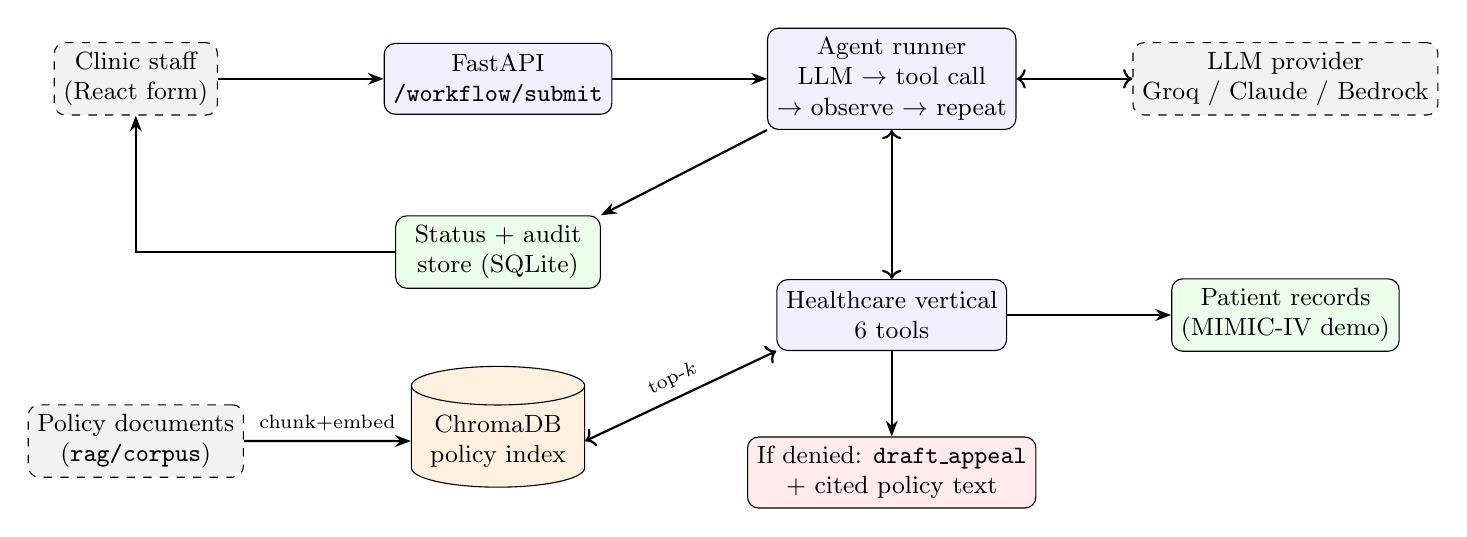
\begin{tikzpicture}[
  node distance=5mm and 9mm,
  box/.style={draw,rounded corners,align=center,minimum height=9mm,minimum width=26mm,font=\small,fill=blue!6},
  store/.style={draw,cylinder,shape border rotate=90,aspect=0.25,align=center,minimum height=11mm,minimum width=22mm,font=\small,fill=orange!12},
  ext/.style={draw,dashed,rounded corners,align=center,minimum height=9mm,font=\small,fill=gray!10},
  arr/.style={-{Stealth[length=2mm]},thick}]
\node[ext] (user) at (0,0) {Clinic staff\\(React form)};
\node[box] (api) at (4.6,0) {FastAPI\\\texttt{/workflow/submit}};
\node[box] (loop) at (9.6,0) {Agent runner\\LLM $\to$ tool call\\$\to$ observe $\to$ repeat};
\node[ext] (llm) at (14.6,0) {LLM provider\\Groq / Claude / Bedrock};
\node[box,fill=green!8] (status) at (4.6,-2.2) {Status + audit\\store (SQLite)};
\node[box] (tools) at (9.6,-3.0) {Healthcare vertical\\6 tools};
\node[store] (vec) at (4.6,-4.6) {ChromaDB\\policy index};
\node[ext] (docs) at (0,-4.6) {Policy documents\\(\texttt{rag/corpus})};
\node[box,fill=green!8] (ehr) at (14.6,-3.0) {Patient records\\(MIMIC-IV demo)};
\node[box,fill=red!8] (appeal) at (9.6,-5.0) {If denied: \texttt{draft\_appeal}\\+ cited policy text};
\draw[arr] (user) -- (api);
\draw[arr] (api) -- (loop);
\draw[arr,<->] (loop) -- (llm);
\draw[arr,<->] (loop) -- (tools);
\draw[arr] (loop.south west) -- (status.north east);
\draw[arr] (status.west) -| (user.south);
\draw[arr] (docs) -- node[above,font=\scriptsize]{chunk+embed} (vec);
\draw[arr,<->] (tools.south west) -- node[above,font=\scriptsize,sloped]{top-$k$} (vec.east);
\draw[arr] (tools) -- (ehr);
\draw[arr] (tools) -- (appeal);
\end{tikzpicture}
\caption{System design. Staff use the chat or submit one form; the agent loop calls tools, retrieves payer policy passages from the vector index, and streams step status back to the UI. A denial triggers a cited appeal draft. Dashed boxes are external to our code; patient records and payer submission are simulated in the current prototype.}
\label{fig:system}
\end{figure*}

\section{System Design}
Figure~\ref{fig:system} shows the components. Two entry points share the retriever: a stateless chat endpoint (tool loop with \texttt{search\_policy}) and the workflow agent. A workflow request flows: UI $\to$ FastAPI (background task) $\to$ agent runner. The runner sends the request and tool schemas to the LLM, executes whichever tool the model selects, appends the observation, and repeats until the model stops calling tools. Tools: \texttt{scan\_insurance\_policy} (RAG), \texttt{analyze\_medical\_records}, \texttt{fill\_authorization\_form}, \texttt{submit\_authorization}, \texttt{track\_authorization\_status}, \texttt{draft\_appeal}. Before the submission tool runs, the loop pauses and the UI shows a review screen; approval resumes it, rejection stops it. Step events and the audit trail are persisted in SQLite and polled by the UI every 1.5\,s.

\textbf{Corpus and scope.} The retrieval index is built from publicly available documents downloaded from their publishers (\texttt{rag/build\_corpus.py}, retrieval date recorded per file): five Aetna Clinical Policy Bulletins (MRI/CT of the spine \cite{aetna0236}, MRI of the extremities, open MRI units, physical therapy, obesity surgery), CMS National Coverage Determination 220.2 (MRI), one Blue Cross Blue Shield of South Carolina lumbar MRI policy, two UnitedHealthcare policies (commercial MRI/CT site of service; Medicare Advantage radiologic diagnostic procedures) and Cigna's site-of-care policy for MRI/CT (whose clinical imaging criteria are delegated to eviCore and absent here); 171 chunks from 10 documents in total. The UnitedHealthcare and Cigna documents contain no lumbar-MRI clinical criteria. Humana and Medicaid documents are not yet included (no fetchable official policy text was found), and the chatbot says so when asked about them. Patient records come from the open MIMIC-IV demo \cite{mimicdemo} (100 real de-identified patients, hospital-admission data only). Payer submission (EDI 278), payer decisions and the structured coverage fields returned by the policy-scan tool are \emph{simulated}.

%-------------------------------------------------------------------------
\section{Methodology}
\label{sec:method}
\textit{Planned for Phase 2 (design only).} (1) \emph{Retrieval}: a set of hand-written queries (payer $\times$ treatment) with labeled relevant passages; metrics Recall@$k$ and MRR, comparing chunk sizes and with/without payer filtering. (2) \emph{Agent trajectory}: for scripted scenarios (approval, denial), check that the tool sequence and arguments are correct across providers; report success rate over repeated runs. (3) \emph{Faithfulness}: fraction of appeal-letter policy claims supported by retrieved passages, judged manually on a sample. (4) \emph{Ablation}: agent with RAG vs.\ static policy dictionary.

\section{Results}
\textbf{Retrieval} (\texttt{eval/retrieval\_eval.py}; 171 chunks from 10 real documents; $n{=}29$ hand-written queries, each labeled with the document that answers it; includes four queries using the exact template the agent issues). With the payer filter, Recall@1/3/5 = 0.86/1.00/1.00 and MRR = 0.92; without it, 0.55/0.86/0.90 and MRR = 0.70. The payer filter therefore matters: without it, other payers' lumbar-MRI policies outrank the Aetna bulletin for Aetna-specific questions. Remaining rank-1 misses are confusions between neighboring Aetna imaging bulletins. Caveat: queries were written by the author after reading the documents, the corpus is small, and the label is document-level, not passage-level, so these numbers are a sanity check, not a benchmark.


\textbf{Real denial cases.} On open data from the California Department of Managed Health Care \cite{dmhc_imr}, we selected the 64 independent medical reviews in which the request was an MRI of the lumbar spine; the reviewer overturned the health plan's denial in 33 of them (52\%). Using only each case's clinical description as the query (cut before any reasoning), retrieval returned a spine-MRI policy (Aetna CPB 0236 or BCBS CAM 709) at rank 1 for 94\% of cases and within the top 3 for 63 of 64, against about 67\% at rank 5 expected by chance. Relevance here is topic-level, not criterion-level, so this shows that retrieval finds the right policy, not that it finds the right criterion.

\textbf{Agent trajectory} (\texttt{eval/agent\_eval.py}; current version with the approval gate auto-approved, a real MIMIC-IV demo patient and the real policy corpus; Groq gpt-oss-120b; 5 runs per scenario). The expected tool sequence was produced in 5/5 standard-approval runs and 5/5 denial-and-appeal runs, with no tool errors, and the appeal cited Aetna CPB 0236. Five runs is a small sample, and an earlier 3-run pilot on a previous version once skipped submission, so the sequence is not guaranteed by the model and we have not enforced it in code. Citation-faithfulness and chat-answer evaluation are pending.

\section{Discussion}
\textit{To be completed in Phase 2.}

\section{Limitations}
Known now: simulated payer interfaces; patient data limited to the 100-patient MIMIC-IV demo (no outpatient notes); small policy corpus (10 documents; Aetna, Medicare, Blue Cross Blue Shield of South Carolina, UnitedHealthcare, Cigna site-of-care only; no Humana or Medicaid); no user authentication or roles (the reviewer name is free text); no HIPAA-grade handling of real PHI (the free LLM tier used here must not receive real patient data); appeal drafts require physician review and the system is not a medical or legal decision-maker. An earlier version indexed hand-written policy entries beside the real documents; they outranked the real Aetna bulletin for generic queries, so they were removed from the index. The retrieval evaluation uses author-written queries, which may favor the documents they were written from.

{\small
\bibliographystyle{ieee_fullname}
\bibliography{refs_medbridge}
}
\end{document}
